% Using my super cool template

\documentclass[13pt,oneside]{tufte-book}

% ams
\usepackage{amssymb,amsmath}

\usepackage{ifxetex,ifluatex}
\usepackage{fixltx2e} % provides \textsubscript
\ifnum 0\ifxetex 1\fi\ifluatex 1\fi=0 % if pdftex
  \usepackage[T1]{fontenc}
  \usepackage[utf8]{inputenc}
\else % if luatex or xelatex
  \makeatletter
  \@ifpackageloaded{fontspec}{}{\usepackage{fontspec}}
  \makeatother
  \defaultfontfeatures{Ligatures=TeX,Scale=MatchLowercase}
  \makeatletter
  \@ifpackageloaded{soul}{
     \renewcommand\allcapsspacing[1]{{\addfontfeature{LetterSpace=15}#1}}
     \renewcommand\smallcapsspacing[1]{{\addfontfeature{LetterSpace=10}#1}}
   }{}
  \makeatother

\fi

% graphix
\usepackage{graphicx}
\setkeys{Gin}{width=\linewidth,totalheight=\textheight,keepaspectratio}

% booktabs
\usepackage{booktabs}

% url
\usepackage{url}

% hyperref
\usepackage{hyperref}

% units.
\usepackage{units}


\setcounter{secnumdepth}{2}

% citations

% pandoc syntax highlighting

% longtable
\usepackage{longtable,booktabs}

% multiplecol
\usepackage{multicol}

% strikeout
\usepackage[normalem]{ulem}

% morefloats
\usepackage{morefloats}


% tightlist macro required by pandoc >= 1.14
\providecommand{\tightlist}{%
  \setlength{\itemsep}{0pt}\setlength{\parskip}{0pt}}

% title / author / date
\title{Information Theory}
\author{Ashwin Reddy}
\date{}

% header-includes
\usepackage{indent first} \usepackage{tikz-cd} \usepackage{algorithm2e}
\usepackage{mdframed} \hypersetup{colorlinks=true, urlcolor=blue}
% end of header-includes

\usepackage{amsthm}
\newtheorem{theorem}{Theorem}[chapter]
\newtheorem{lemma}{Lemma}[chapter]
\newtheorem{corollary}{Corollary}[chapter]
\newtheorem{proposition}{Proposition}[chapter]
\newtheorem{conjecture}{Conjecture}[chapter]
\theoremstyle{definition}
\newtheorem{definition}{Definition}[chapter]
\theoremstyle{definition}
\newtheorem{example}{Example}[chapter]
\theoremstyle{definition}
\newtheorem{exercise}{Exercise}[chapter]
\theoremstyle{remark}
\newtheorem*{remark}{Remark}
\newtheorem*{solution}{Solution}
\let\BeginKnitrBlock\begin \let\EndKnitrBlock\end
\begin{document}

{
\surroundwithmdframed{theorem}
\surroundwithmdframed{example}
\surroundwithmdframed{exercise}
}

\maketitle


% include befores
% end of include befores

{
\setcounter{tocdepth}{1}
\tableofcontents
}

\listoftables
\listoffigures

\chapter{Introduction}\label{introduction}

Often, lecture notes like these jump into the material without
establishing the basics. This chapter will cover why this book exists
and how to use it.

\section{Philosophy}\label{philosophy}

Two other sets of notes for this course are available at
\url{https://github.com/mananshah99/infotheory} and
\url{http://tiny.cc/infotheory1} . My goal in preparing \emph{this} book
was simply to ensure that I understand the concepts. As a result, I've
spared no expense in filling these notes with as much content as needed
to develop the theory from first principles.

It's also worth noting that the stylistic choices I've made here are
very opinionated. The margins are very wide and are filled with
important asides and footnotes. I've tried to stick to the typical
definition-theorem-proof style with explanatory prose in between.
Speaking of color, you've probably noticed that URLs are in blue.

\section{Prerequisites}\label{prerequisites}

This book assumes a proficiency with single-variable calculus and some
familiarity with multivariable calculus. Important concepts of
probability are developed from scratch, however.

\section{Why study Information
Theory?}\label{why-study-information-theory}

Information Theory is a mathematical framework for thinking about what
it means to have efficient communication. Examples of information
include:

\begin{itemize}
\tightlist
\item
  Email
\item
  Telegraph
\item
  Images
\item
  Speech
\item
  Video
\end{itemize}

Much of today's digital world revolves around transmitting information:
we zip files, email them across the internet, download MP3s, etc. The
ideas of information theory give us a rigorous way of characterizing
streams of information. The cornerstone of our model will start with the
following pipeline of sorts

\begin{figure}
\centering
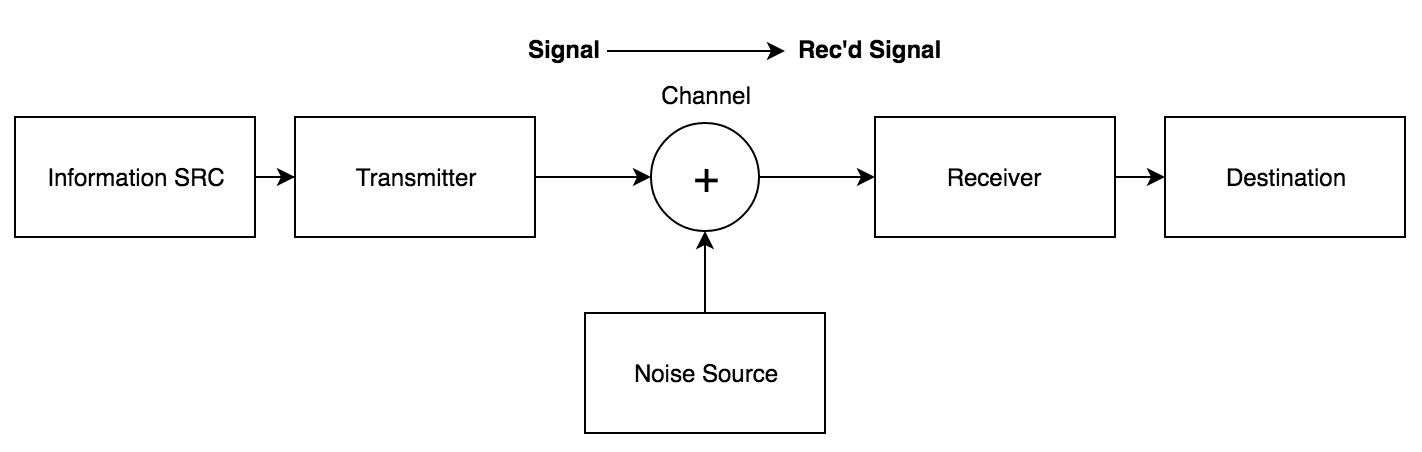
\includegraphics{pipeline.png}
\caption{}
\end{figure}

This model gives us a general way of abstracting the transmission of
information. On the left we have a source of information (where a signal
originates) that is sent to a transmitter. A channel then allows that
signal to flow to a receiver, although noise may be added at this stage.
Finally, the receiver sends the signal to the destination. Right now,
this model may not be very elucidating. However, we will see that it
gives us a structure within which we can consider various mathematical
characterizations of information. However, before we can begin to
consider information in depth, we must first start our foundation with a
solid understanding of probability as that is the underlying theory
below Information Theory.

\part{Theory}\label{part-theory}

\chapter{Stochastic Variables}\label{stochastic-variables}

\BeginKnitrBlock{definition}[Stochastic Variable]
\protect\hypertarget{def:unnamed-chunk-1}{}{\label{def:unnamed-chunk-1}
\iffalse (Stochastic Variable) \fi{} } A \textbf{stochastic variable} is
a real-valued function of an outcome of an experiment.
\EndKnitrBlock{definition}

\BeginKnitrBlock{remark}
\iffalse{} {Remark. } \fi{} Stochastic variables are also called random
variables, but this term seems to imply all possibilities are equally
likely or cannot be determined. The word stochastic generally means
something like ``depending upon probabilities.''
\EndKnitrBlock{remark}

\BeginKnitrBlock{example}
\protect\hypertarget{exm:unnamed-chunk-3}{}{\label{exm:unnamed-chunk-3} }
Toss a coin 7 times. The number of heads in the sequence could be a
stochastic variable.
\EndKnitrBlock{example}

\BeginKnitrBlock{remark}
\iffalse{} {Remark. } \fi{} The 7-long sequence itself is not a
stochastic variable, since it is not a real value. We should always have
a clear way of assigning a real number to the outcome.
\EndKnitrBlock{remark}

\BeginKnitrBlock{example}
\protect\hypertarget{exm:unnamed-chunk-5}{}{\label{exm:unnamed-chunk-5} }
Sum two rolls of a die. This value could be a stochastic variable. The
number of 5's rolled could also be a stochastic variable.
\EndKnitrBlock{example}

A stochastic variable can either be discrete, taking on values from a
countable set or continuous, taking on values on an interval from the
real number line.

\section{Probability Measure}\label{probability-measure}

\BeginKnitrBlock{definition}[Sample Space]
\protect\hypertarget{def:unnamed-chunk-6}{}{\label{def:unnamed-chunk-6}
\iffalse (Sample Space) \fi{} } The sample space is the set of all
possible outcomes for an experiment.
\EndKnitrBlock{definition}

\begin{marginfigure}
The sample space is typically denoted as \(\Omega\).
\end{marginfigure}

\BeginKnitrBlock{definition}[Event]
\protect\hypertarget{def:unnamed-chunk-8}{}{\label{def:unnamed-chunk-8}
\iffalse (Event) \fi{} } An \textbf{event} is a subset of the sample
space \(\Omega\).
\EndKnitrBlock{definition}

\BeginKnitrBlock{remark}
\iffalse{} {Remark. } \fi{} Any event belongs to the power set of
\(\Omega\).\footnote{The Wikipedia article on
  \href{https://en.wikipedia.org/wiki/Event_(probability_theory)\#A_simple_example}{events}
  has good examples.} Thus, events range from the empty set to a
singleton set (i.e.~a set with size unity) to \(\Omega\) itself and
anything in between.
\EndKnitrBlock{remark}

\begin{marginfigure}
\begin{tikzcd}
 & X \arrow{dr}{\text{can take on values from}} \\
\mathbb{P} \arrow{ur}{\text{function of}} \arrow{rr}{\text{of specific value}} && x
\end{tikzcd}
\end{marginfigure}

\BeginKnitrBlock{definition}[Probability Measure]
\protect\hypertarget{def:unnamed-chunk-11}{}{\label{def:unnamed-chunk-11}
\iffalse (Probability Measure) \fi{} } The probability measure
\(\mathbb{P}\) is a real-valued function that assigns events
probabilities obeying the Kolmogorov axioms.
\EndKnitrBlock{definition}

Our notions of probability are fairly intuitive, so a careful treatment
of the Kolmogorov axioms is not needed. They are available in the
\protect\hyperlink{kmaxm}{appendix}, however.

\begin{marginfigure}
\textbf{Notation}. In general, if \(X\) is a stochastic variable, the
probability mass function can be written in two equivalent ways:

\begin{equation}
p_X(x) = \mathbb{P}(X=x)
\label{eq:prob-notation}
\end{equation}
\end{marginfigure}

\section{Bayes' Theorem}\label{bayes-theorem}

When events \(A\) and \(B\) are not independent, knowing what \(A\) is
gives us information about what \(B\) might be (and vice versa). The
notation \(\mathbb{P}(A|B)\) denotes the probability of \(A\) given that
or conditioned upon \(B\) occuring. Consider that for \(A\) and \(B\) to
happen that \(B\) must first happen and \(A\) must happen under those
circumstances.

\[
\mathbb{P}(A \cap B)  = \mathbb{P}(B) \cdot \mathbb{P}\left(A | B\right) 
\]

From this definition, Thomas Bayes determined how to compute the support
\(B\) provides for \(A\) given \emph{priors} and \emph{posteriors}.

\BeginKnitrBlock{theorem}[Bayes' Theorem]
\protect\hypertarget{thm:unnamed-chunk-13}{}{\label{thm:unnamed-chunk-13}
\iffalse (Bayes' Theorem) \fi{} }

\begin{equation}
\mathbb{P}( A|B) = \frac{\mathbb{P}(B|A)\mathbb{P}(A)}{\mathbb{P}(B)}
\end{equation}
\EndKnitrBlock{theorem}

\section{Probability Mass Functions}\label{probability-mass-functions}

A \textbf{probability mass function} (pmf) characterizes a discrete
stochastic variable by returning the probability measure of some \(x\)
in \(\Omega\) occuring.

\BeginKnitrBlock{example}
\protect\hypertarget{exm:unnamed-chunk-14}{}{\label{exm:unnamed-chunk-14} }
Consider 2 tosses of a fair coin. What is the probability mass function
(pmf) of the number of heads given this experiment?
\EndKnitrBlock{example}

\BeginKnitrBlock{solution}
\iffalse{} {Solution. } \fi{} It is useful to construct a table of all
the possibilities.

\begin{longtable}[]{@{}lll@{}}
\toprule
& Heads & Tails\tabularnewline
\midrule
\endhead
Heads & 2 & 1\tabularnewline
Tails & 1 & 0\tabularnewline
\bottomrule
\end{longtable}

From the table, we can conclude that

\[
\mathbb{P}(X=x) = \begin{cases}
1/4 & x = 0 \\
1/2 & x = 1 \\
1/4 & x = 2 \\
0 & \text{otherwise}
\end{cases}
\]
\EndKnitrBlock{solution}

\BeginKnitrBlock{example}
\protect\hypertarget{exm:unnamed-chunk-16}{}{\label{exm:unnamed-chunk-16} }
Consider a 4-sided die rolled twice. What is the probability mass
function for the maximum value of 2 rolls?
\EndKnitrBlock{example}

\BeginKnitrBlock{solution}
\iffalse{} {Solution. } \fi{}

As before, let us think about the various possibilities. There are
\(4 \times 4 = 16\) total possibilities, and the maximum value can take
on values 1, 2, 3, and 4. To take on a value of 1, both rolls must have
been a 1; the probability of this happening is 1/16. To take on a value
of 2, one of the rolls must have been a 2 and the other one must have
been a 1 or a 2. The possibilites are enumerated as (2,1), (2,2), (1,2).
Thus, its chance is 3/16. For a max value of 3, the possibilities are
(3,1), (3,2), (3,3), (1,3), (2,3). Thus,

\[
p_X(x) = \begin{cases}
1/16 & x = 1 \\
3/16 & x = 2 \\
5/16 & x = 3 \\
7/16 & x = 4 \\
0 & \text{otherwise}
\end{cases}
\]
\EndKnitrBlock{solution}

There are a few common discrete stochastic variables that are worth
discussing separately. The chapter on
\protect\hyperlink{discrete-stochastic-variables}{Discrete Stochastic
Variables} covers 4 important ones. The following sections will assume
familiarity with these variables.

\section{Expectation and Variance}\label{expectation-and-variance}

As is often the case in mathematics, we like to define general operators
on objects to understand their properties. Firstly, note that we can use
functions of stochastic variables to build other stochastic variables.

\BeginKnitrBlock{example}[Simple Functions of a Stochastic Variable]
\protect\hypertarget{exm:unnamed-chunk-18}{}{\label{exm:unnamed-chunk-18}
\iffalse (Simple Functions of a Stochastic Variable) \fi{} }Consider the
following pmf

\[
p_X(x) = \begin{cases}
1/9 & x \in \{ -4, -3, -2, -1, 0, 1, 2, 3, 4\} \\
0 & \text{otherwise}
\end{cases}
\] Here are two functions of \(X\) and their probability mass functions:

\begin{enumerate}
\def\labelenumi{\alph{enumi})}
\tightlist
\item
  \(Y=|X| \implies p_Y(y)=\begin{cases}2/9 & y \in \{1,2,3,4\} \\ 1/9 & y=0 \end{cases}\)
\item
  \(Z=X^2 \implies p_Z(z)=\begin{cases}2/9 & z \in \{1,4,9,16\} \\ 1/9 & z=0 \end{cases}\)
\end{enumerate}
\EndKnitrBlock{example}

A special class of functions, known as moments, include two operators,
\textbf{expectation} and \textbf{variance}.

\BeginKnitrBlock{definition}[Expectation]
\protect\hypertarget{def:unnamed-chunk-19}{}{\label{def:unnamed-chunk-19}
\iffalse (Expectation) \fi{} } The expectation of a function \(g\) of a
stochastic variable \(X\) is

\[
\mathbb{E}[g(X)] \equiv \sum_{x \in \Omega} g(x) \cdot \mathbb{P}(X=x)
\]
\EndKnitrBlock{definition}

\BeginKnitrBlock{theorem}[Linearity of Expectation]
\protect\hypertarget{thm:unnamed-chunk-20}{}{\label{thm:unnamed-chunk-20}
\iffalse (Linearity of Expectation) \fi{} }\[
\mathbb{E}\left[aX+bY\right] = a\mathbb{E}[X]+b\mathbb{E}[Y]
\]
\EndKnitrBlock{theorem}

\begin{marginfigure}
The \(n\)th moment about \(x_0\) is defined as
\(\mathbb{E}[(x-x_0)^n]\).
\end{marginfigure}

\BeginKnitrBlock{definition}[Variance]
\protect\hypertarget{def:unnamed-chunk-22}{}{\label{def:unnamed-chunk-22}
\iffalse (Variance) \fi{} } The variance is the 2nd moment about the
mean.

\begin{equation}
\mathrm{Var}[X] \equiv \mathbb{E}[(X-\mathbb{E}[X])^2]
\label{eq:variance-def}
\end{equation}
\EndKnitrBlock{definition}

Unfortunately, the definition given above in Equation
\eqref{eq:variance-def} tends to be difficult to compute by hand. A little
algebra results in a computationally simpler alternative.

\BeginKnitrBlock{lemma}[Determinism of Expectation of Expectation]
\protect\hypertarget{lem:unnamed-chunk-23}{}{\label{lem:unnamed-chunk-23}
\iffalse (Determinism of Expectation of Expectation) \fi{} }\[
\mathbb{E}\Big[\mathbb{E}[X]\Big] = \mathbb{E}[X]
\]
\EndKnitrBlock{lemma}

\BeginKnitrBlock{theorem}[Computationally Simpler Alternative for Variance]
\protect\hypertarget{thm:unnamed-chunk-24}{}{\label{thm:unnamed-chunk-24}
\iffalse (Computationally Simpler Alternative for Variance) \fi{} }

\begin{equation}
\mathrm{Var}[X] = \mathbb{E}[X^2] - \mathbb{E}\left[X\right]^2
\label{eq:variance-comp}
\end{equation}
\EndKnitrBlock{theorem}

\BeginKnitrBlock{proof}
\iffalse{} {Proof. } \fi{}

\begin{align*}
\mathrm{Var}[X] &= \mathbb{E}\Big[X^2 + \mathbb{E}[X]^2 - 2X\mathbb{E}[X]\Big] \\
&= \mathbb{E}[X^2] + \mathbb{E}[X]^2 - 2\mathbb{E}[X]\mathbb{E}[X] \\
&= \mathbb{E}[X^2] - \mathbb{E}[X]^2.
\end{align*}
\EndKnitrBlock{proof}

\begin{marginfigure}
As an aside, the indicator function \(\mathbb{1}_A\) indicates whether
certain events are in \(A\) or not.

\[
\mathbb{1}_A(\omega) = \begin{cases} 1 & \omega \in A \\ 0 & \omega \not\in A \end{cases}
\]

As a result,

\[\mathbb{E}[\mathbb{1}_A(\omega)] = \mathbb{P}(A)\]
\[\mathrm{Var}[\mathbb{1}_A(\omega)] = P(A)(1-P(A))\]
\end{marginfigure}

\begin{longtable}[]{@{}lll@{}}
\caption{Expectation and Variance of Common
Distributions}\tabularnewline
\toprule
Distribution & Expectation & Variance\tabularnewline
\midrule
\endfirsthead
\toprule
Distribution & Expectation & Variance\tabularnewline
\midrule
\endhead
Binomial & \(np\) & \(np(1-p)\)\tabularnewline
Geometric & \(1/p\) & \((1-p)/p^2\)\tabularnewline
Poisson & \(\lambda\) & \(\lambda\)\tabularnewline
\bottomrule
\end{longtable}

\section{Probability Density
Functions}\label{probability-density-functions}

Now we turn to stochastic variables that return values on an interval of
the real number line. We can use our knowledge of discrete stochastic
variables to find analagous versions for continuous stochastic
variables. Instead of a probability mass function, we call the function
for a continuous stochastic variables \textbf{probability density
function} (pdf).

\begin{marginfigure}
\textbf{Notation}. Probability density functions are typically denoted
with lowercase English letters, most commonly \(f\).
\end{marginfigure}

The requirement that the total probability must add up to unity is still
in place:

\[
\int_{\mathbb{R}} f_X(x)\,\mathrm{d}x=1
\]

However, asking whether \(X=x\) is no longer a well-formed question,
since \(X\) has a continuum. The probability that \(X\) takes on the
exact value \(x\) is nil. Therefore, probabilities of a continuous
stochastic variable may only be queried in the following form.

\[
\mathbb{P}(a\leq X \leq b) = \int\limits_{a}^{b}f_X(x)\,\mathrm{d}x
\]

By extension, the expectation of a pdf can be computed as

\[
\mathbb{E}[X] = \int_{\mathbb{R}}xf_X(x)\,\mathrm{d}x
\]

The chapter on
\protect\hyperlink{continuous-stochastic-variables}{Continuous
Stochastic Variables} discusses 3 important stochastic variables:
uniform, exponential, and Gaussian. These variables will come up later,
but for the sake of cleanliness, the proofs and computations have been
moved into the appendix.

\chapter{Entropy}\label{entropy}

Why did we spend the time reviewing probability for information? The
answer lies in Proposition \ref{prp:stochasticity-of-info} below:

\BeginKnitrBlock{proposition}[Stochasticity of Information]
\protect\hypertarget{prp:stochasticity-of-info}{}{\label{prp:stochasticity-of-info}
\iffalse (Stochasticity of Information) \fi{} } Information can be
modelled as samples from a stochastic source.
\EndKnitrBlock{proposition}

Consider the fact that many emails you send will have a typical
structure: a greeting, a body of text, a conclusion. Or that the changes
in the frames of a video tend to be rather small. Intuitively, we have a
sense that the repetitive elements of data are not information-dense,
and therefore, when we transmit this information, we should really only
focus on what is novel about each message.

Shannon's original example was to show that text can modelled
probabilistically in this way. Let's imagine that we want to generate
some text that looks like English. We can first start by creating a
sample space \(\Omega\) that includes letters and spaces. Then, we
sample randomly. This is callled a zero-order approximation. Next, we
can refine the approximation by making characters more or less frequent.
Adapting the probability based on the frequency with which that
character appears in a corpus (e.g.~make \emph{e} show up about 12\% of
the time) is called a first-order approximation. An even more refined
approach would consider digram (2-character sequences) and their
frequencies.

\section{Surprisal}\label{surprisal}

Now that you're convinced that information can be modelled
stochastically, we can consider what information means.

\BeginKnitrBlock{example}[The Q-U Question]
\protect\hypertarget{exm:unnamed-chunk-28}{}{\label{exm:unnamed-chunk-28}
\iffalse (The Q-U Question) \fi{} } Consider a game where you predict
the next letter of a piece of English text given all the previous
letters. You are given the phrase \texttt{elephants\ are\ q}. You know
that the letter \texttt{q} is nearly always followed by a \texttt{u}.
You would then predict that the next letter is a \texttt{u}, and you
would be confident in your guess. If, by some odd reason, that next
letter is not a \texttt{u}, you would be ``surprised''.
\EndKnitrBlock{example}

What we've captured in this example is a working conception of
information.

\BeginKnitrBlock{definition}[Information]
\protect\hypertarget{def:unnamed-chunk-29}{}{\label{def:unnamed-chunk-29}
\iffalse (Information) \fi{} } New information (which is really the only
kind of information we care about) \textbf{is} the ``surprisal'' of an
information source. The more surprised you are, the more information you
gain, since you didn't expect to see that result.
\EndKnitrBlock{definition}

We now need a way of quantifying surprisal/information. The core of our
theory is that surprisal should be inversely correlated with the
probability of occurence. So naturally, we gravitate towards picking
something like \(1/p\) as our information function. Consider the limit
cases, however, of literally using \(1/p\). When \(p=0\), we have
infinite surprisal, and when \(p=1\), we have 1 unit of surprisal. If
something is guaranteed to happen, 1 unit is an odd baseline to use. As
a result, we pick \(\log(1/p)\), which is more attractive for a few
reasons.

\begin{enumerate}
\def\labelenumi{\arabic{enumi}.}
\tightlist
\item
  Continuity
\item
  Monotonically decreasing in \(p\)
\item
  Never negative
\item
  With \(p=1\), information becomes 0
\item
  Information due to independent events is additive
\end{enumerate}

\begin{marginfigure}
Which base we pick is entirely arbitrary as long as it makes sense
(sensible options include 2, 10, and \(e\)). The value of entropy
changes predictably with a change of base, so it really doesn't pose
much of a problem. In most cases, we will pick base 2, since we like to
consider binary digits (abbreviated bits).
\end{marginfigure}

To each event, we now attach a surprisal value. To characterize a
stochastic variable as a whole, we now define entropy.

\BeginKnitrBlock{definition}[Entropy]
\protect\hypertarget{def:unnamed-chunk-31}{}{\label{def:unnamed-chunk-31}
\iffalse (Entropy) \fi{} } The entropy \(H\) of a stochastiv variable
\(X\) is the expectation of surprisal of \(X\).

\begin{align*}
H(X) &\equiv \mathbb{E}\left[\log \frac{1}{\mathbb{P}(X=x)}\right]\\
&= \sum_i p_i \log(1/p_i) \\
&= -\sum_i p_i \log p_i
\end{align*}
\EndKnitrBlock{definition}

\begin{marginfigure}
Shannon's formula for entropy actually has a similarity to thermodynamic
entropy:

\[
S = - k_B \sum p_i \ln p_i
\]
\end{marginfigure}

\BeginKnitrBlock{example}[Entropy of Bernoulli Distribution]
\protect\hypertarget{exm:unnamed-chunk-33}{}{\label{exm:unnamed-chunk-33}
\iffalse (Entropy of Bernoulli Distribution) \fi{} }\[
H(X) = p \log \frac{1}{p} + (1-p)\log \frac{1}{1-p}
\]
\EndKnitrBlock{example}

Plotting for every possible value for \(p\), we yield a nice graph:

\begin{figure}
\includegraphics{_main_files/figure-latex/unnamed-chunk-34-1} \caption[Bernoulli Entropy]{Bernoulli Entropy}\label{fig:unnamed-chunk-34}
\end{figure}

When \(p\) is 0 or 1, we need 0 bits of information, which makes sense
because the result was guaranteed. As we go more towards complete
randomness (which colloquially, we might also call ``entropy'' from a
physics standpoint), we need more bits to represent the possibilites (a
maximum of 1 in this case).

But what does it mean to have 0.47 bits, which we might have if
\(p(\text{heads})=0.9\)? Imagine that we had a 100-long sequence of coin
flips and we transmitted the information. For the purely random case
(i.e.~using a fair coin), we would need 100 bits. However, for this
extremely unfair case, we could get away with 47 bits without losing any
information (on average).

\section{Bit Representations}\label{bit-representations}

While we will be overloading the word bit in different contexts in this
book, it is useful to understand what it represents. As noted before,
bit is an abbreviation of ``binary digit.'' When we talk about a bit in
computer science, we typically mean 0 or 1, low voltage or high voltage,
etc. Here, we take a bit to mean something like the answer to a single
yes or no question with yes and no equally likely. In other words, a
coin toss. That is, one bit captures the information of a Bernoulli
distribution with \(p=0.5\). From there, we can meaningfully interpret
values of entropy as telling us roughly how many of these yes/no
questions or coin flips or sequence of binary digits are needed to
transmit the information on average.

\BeginKnitrBlock{example}[Entropy of a Fair Dice Roll]
\protect\hypertarget{exm:fair-dice-roll}{}{\label{exm:fair-dice-roll}
\iffalse (Entropy of a Fair Dice Roll) \fi{} } Find the entropy of a
fair dice roll.
\EndKnitrBlock{example}

\BeginKnitrBlock{solution}
\iffalse{} {Solution. } \fi{}

Note that entropy does not care about the actual values of \(X\).
Therefore, the entropy is computed as

\begin{align*}
H(x) &= \sum_x p(x)\log(1/p(x)) \\
&= \sum_{x=1}^6 \frac{1}{6}\log(6) \\
&= 6\cdot\frac{1}{6}\log(6) \\
&= \log 6 \approx 2.585
\end{align*}
\EndKnitrBlock{solution}

\BeginKnitrBlock{exercise}[Double the Possibilities]
\protect\hypertarget{exr:unnamed-chunk-36}{}{\label{exr:unnamed-chunk-36}
\iffalse (Double the Possibilities) \fi{} } Repeat Example
\ref{exm:fair-dice-roll} except that there are double the number of
possible values (i.e.~a 12-sided die).
\EndKnitrBlock{exercise}

\BeginKnitrBlock{solution}
\iffalse{} {Solution. } \fi{} Intuitively, we just need to add one more
bit to flip between the first 6 and last 6 values. Mathematically, we
consider \(\log(12)\), which by log properties is
\(\log(2) + \log(6) = 1 + \log(6)\).
\EndKnitrBlock{solution}

\section{Jensen's Inequality}\label{jensens-inequality}

\BeginKnitrBlock{definition}[Convex Function]
\protect\hypertarget{def:unnamed-chunk-38}{}{\label{def:unnamed-chunk-38}
\iffalse (Convex Function) \fi{} } A function \(f(x)\) is convex on the
interval \((a,b)\) if it is concave up on that interval (i.e.~second
derivative is positive). Alternatively, it obeys the property that for
all \((x_1, x_2)\) within the interval \((a,b)\) and for all \(\lambda\)
normalized between 0 and 1,

\[
f(\lambda x_1 + (1-\lambda)x_2) \leq \lambda f(x_1) + (1-\lambda) f(x_2)
\]
\EndKnitrBlock{definition}

\BeginKnitrBlock{theorem}[Jensen's Inequality]
\protect\hypertarget{thm:unnamed-chunk-39}{}{\label{thm:unnamed-chunk-39}
\iffalse (Jensen's Inequality) \fi{} }For a stochastic variable \(X\)
and a function \(f\),

\[
\mathbb{E}[f(X)] \geq f(\mathbb{E}[X])
\]
\EndKnitrBlock{theorem}

\BeginKnitrBlock{theorem}
\protect\hypertarget{thm:unnamed-chunk-40}{}{\label{thm:unnamed-chunk-40}
}If \(X\) assumes real values \(\{x_1, \dots, x_n\}\) and
\(0 \leq H(X) \leq \log r\). Then,

\[
\forall\, 1 \leq i \leq n,  p_i = \frac{1}{r} \iff  H(X)=\log r 
\]
\EndKnitrBlock{theorem}

\section{Joint Entropy}\label{joint-entropy}

\BeginKnitrBlock{definition}[Joint Entropy]
\protect\hypertarget{def:unnamed-chunk-41}{}{\label{def:unnamed-chunk-41}
\iffalse (Joint Entropy) \fi{} }\[
H(X,Y) = -\sum_{x}\sum_{y} \mathbb{P}(x,y)\log(p(x,y))
\]
\EndKnitrBlock{definition}

\BeginKnitrBlock{definition}[Conditional Entropy]
\protect\hypertarget{def:unnamed-chunk-42}{}{\label{def:unnamed-chunk-42}
\iffalse (Conditional Entropy) \fi{} }\[
H(Y | X) = \sum_x p(x) H(Y | X = x)
\]
\EndKnitrBlock{definition}

\BeginKnitrBlock{theorem}
\protect\hypertarget{thm:unnamed-chunk-43}{}{\label{thm:unnamed-chunk-43} }

\begin{align*}
H(X,Y) &= H(X) + H(Y  | X) \\
&= H(Y) + H(X | Y)
\end{align*}
\EndKnitrBlock{theorem}

\BeginKnitrBlock{proof}
\iffalse{} {Proof. } \fi{}
\EndKnitrBlock{proof}

\section{Differential Entropy}\label{differential-entropy}

Differential entropy is the continuous version of discrete entropy.

\BeginKnitrBlock{proof}
\iffalse{} {Proof. } \fi{} The probability that \(X^\Delta\) is in the
\(i\)th bin is \(p(x_i)\Delta x\). Then,

\begin{align*}
H(X^\Delta) &= - \sum_i p(x_i) \Delta x \log\left(p(x_i)\Delta x\right) \\
&= \sum_i \left[ p(x_i)\Delta x \log \frac{1}{p(x_i)} + p(x_i)\Delta x \log \frac{1}{\Delta x} \right]
\end{align*}
\EndKnitrBlock{proof}

\[
h(x) \equiv -\int_{\mathbb{R}} f(x)\log f(x) \,\mathrm{d}x
\]
\BeginKnitrBlock{example}[Differential Entropy of Uniform Stochastic Variable]
\protect\hypertarget{exm:unnamed-chunk-46}{}{\label{exm:unnamed-chunk-46}
\iffalse (Differential Entropy of Uniform Stochastic Variable) \fi{} }
On the interval \([0,a]\),

\[
h(x) = \int\limits_0^a \frac{1}{a} \log a \,\mathrm{d}x = \log a
\]
\EndKnitrBlock{example}

Notice that if \(a \leq 1\), we have 0 and negative values of entropy,
so differential entropy really isn't like discrete entropy.

\chapter{Source Coding}\label{source-coding}

\section{Encoding the English
Alphabet}\label{encoding-the-english-alphabet}

Here's a practical problem we would like to solve: Given the 26 letters
of the English alphabet and assuming letters are coming independently,
design an encoder (a schema that converts text into a binary message) to
minimize the expected number of bits used per letter. Essentially, can
we find an encoding of the English alphabet using a zero-order
approximation?

We'll start with a simple solution:

\begin{enumerate}
\def\labelenumi{\arabic{enumi}.}
\tightlist
\item
  Compute how many bits it would take if each letter had the same number
  of bits. The number of bits needed is given by
  \(\lceil \log_2(26)\rceil\)\footnote{The upper brackets denote the
    ceiling function or greatest integer function. The number of bits
    must be a natural number.}
\item
  Then, \emph{A} becomes \texttt{00000}, \emph{B} becomes
  \texttt{00001}, and so on and so forth.
\item
  Store the characters and their numbers in a matrix. The matrix serves
  as both the encoding and decoding scheme.
\end{enumerate}

Solution \#1 is actually the best approach if each character had an
equal probability (i.e. \(1/26\)) of appearing. However, certain
characters tend to appear more than others. Therefore, using the same
number of bits to represent a commonly occuring character like \emph{e}
and a infrequent character like \emph{z} is not making the best use of
each bit.

Our next solution will take into account frequency. The three most
common letters in the English alphabet are \emph{E}, \emph{T}, and
\emph{A}. Assign \emph{E} the value \texttt{0}, \emph{T} the value
\texttt{1}, and \emph{A} the value \texttt{10}. However, it now becomes
impossible to determine whether \texttt{10} is a ``TA'' message or an
``E'' message. We need to avoid such prefix-collisions to interpret
messages without ambiguity.

\section{Huffman Coding}\label{huffman-coding}

The solution devised by David Huffman has optimality given certain
conditions. First, we'll need to describe the algorithm of Huffman
coding.

\begin{algorithm}[H]
    \SetAlgoLined
    \KwData{A map $m: \Sigma \to [0,1]$}
    \KwResult{A binary tree representing an encoding scheme}
    \While{$|\mathrm{preimage}(m)| > 1$}{
        $a \gets \arg\min m$\;
        Remove $a$ from $m$\;
        $b \gets \arg\min m$\;
        Remove b from $m$\;
        Insert symbol $ab$ with frequency $m(a)+m(b)$\;
    }
\caption{Huffman Coding}
\end{algorithm}

\BeginKnitrBlock{theorem}[Huffman Coding Optimality]
\protect\hypertarget{thm:unnamed-chunk-47}{}{\label{thm:unnamed-chunk-47}
\iffalse (Huffman Coding Optimality) \fi{} } If \(X\) is a random
variable, and \(L\) is the expected number of bits per letter using
Huffman coding,

\[
H(X) \leq L \leq H(X)+1
\]
\EndKnitrBlock{theorem}

An intuitive video explaining Huffman coding can be found here:
\url{https://www.youtube.com/watch?v=JsTptu56GM8} . A Python program is
available here:
\url{https://gist.github.com/ashwinreddy/8b8eb194bc3bf264a81affb5b6cdff06}
.

\part*{Appendix}\label{part-appendix}
\addcontentsline{toc}{part}{Appendix}

\appendix


\hypertarget{discrete-stochastic-variables}{\chapter{Discrete Stochastic
Variables}\label{discrete-stochastic-variables}}

\section{Bernoulli Distribution}\label{bernoulli-distribution}

A Bernoulli distribution represents the number of heads in tossing a
potentially unfair coin once. The unfairness is characterized by a
probability \(p\) that the coin lands heads. Therefore, the probability
that the coin lands tails is \(1-p\).

\BeginKnitrBlock{definition}[Bernoulli Distribution]
\protect\hypertarget{def:unnamed-chunk-48}{}{\label{def:unnamed-chunk-48}
\iffalse (Bernoulli Distribution) \fi{} }

\begin{equation}
\mathrm{Bern}(x) \equiv \begin{cases}
p & x = 1 \\
1-p & x = 0
\end{cases}
\end{equation}
\EndKnitrBlock{definition}

\section{Binomial Distribution}\label{binomial-distribution}

Next, the binomial distribution can be imagined as tossing the same
unfair coin \(N\) times and counting the number of heads. The
probability that the number of heads is nil is \((1-p)^N\) since the
implication is that the coin came up tails every single time. The
probability that the number of heads is exactly one is
\(Np(1-p)^{N-1}\). This is because it must have come up heads once with
probability \(p\) and tails \(N-1\) times with probability \(1-p\).
Additionally, the one heads could come up at any point in the sequence,
which introduces a factor of \(\binom{N}{k}\).

\BeginKnitrBlock{definition}[Binomial Distribution]
\protect\hypertarget{def:unnamed-chunk-49}{}{\label{def:unnamed-chunk-49}
\iffalse (Binomial Distribution) \fi{} }

\begin{equation}
\mathbb{P}(X=k; n, p) \equiv \binom{n}{k} p^k (1-p)^{n-k}
\end{equation}
\EndKnitrBlock{definition}

You can check that \(\mathbb{P}(X=1; 1, p) = \mathrm{Bern}(p)\)

\section{Geometric Distribution}\label{geometric-distribution}

In a geometric distribution, we keep tossing the coin until there is one
heads.

\BeginKnitrBlock{definition}[Geometric Distribution]
\protect\hypertarget{def:unnamed-chunk-50}{}{\label{def:unnamed-chunk-50}
\iffalse (Geometric Distribution) \fi{} }

\begin{equation}
p_X(x) = (1-p)^{x-1}p
\end{equation}
\EndKnitrBlock{definition}

\section{Poisson Distribution}\label{poisson-distribution}

\BeginKnitrBlock{definition}[Poisson Distribution]
\protect\hypertarget{def:unnamed-chunk-51}{}{\label{def:unnamed-chunk-51}
\iffalse (Poisson Distribution) \fi{} } \[
p_X(x = k) = \frac{\lambda^k}{k!}e^{-\lambda}.
\]
\EndKnitrBlock{definition}

Similar to a binomial distribution, the Poisson distribution can be
thought of as the number of replacements needed for a biased lightbulb
(rather than a coin) in a given amount of time. In this case, we are
typically dealing with a large \(n\) and a small \(p\), which leads to a
``moderate'' \(np\).\footnote{I have no idea what this means.} If
\(\lambda \equiv np\) (can be thought of as the expected number of times
the bulb will burn out),

\BeginKnitrBlock{proof}
\iffalse{} {Proof. } \fi{} Start with binomial distribution, using
\(\lambda\) instead of \(p\):

\begin{align*}
p_X(x=k) &= \lim_{n\to\infty}\lim_{p\to 0} \frac{n!}{(n-k)!k!}\binom{\lambda}{n}^k\left(1-\frac{\lambda}{n}\right)^{n-k} \\
&= \lim_{n\to\infty}\lim_{p\to 0} \frac{n(n-1)\dots (n-k+1)}{n^k}\cdot\frac{\lambda^k}{k!}\frac{(1-\lambda/n)^n}{(1-\lambda/n)^k)} \\
&= e^{-\lambda}\lambda^k/k!
\end{align*}
\EndKnitrBlock{proof}

\begin{marginfigure}
What can be modelled with a Poisson distribution?

\begin{itemize}
\tightlist
\item
  Number of customers entering a bank in a given period of time
\item
  Number of misprints on a page
\item
  Number of alpha particles discharged from a radioactive substance.
\end{itemize}
\end{marginfigure}

\hypertarget{continuous-stochastic-variables}{\chapter{Continuous
Stochastic Variables}\label{continuous-stochastic-variables}}

\section{Uniform}\label{uniform}

\BeginKnitrBlock{definition}[Uniform Stochastic Variable]
\protect\hypertarget{def:unnamed-chunk-54}{}{\label{def:unnamed-chunk-54}
\iffalse (Uniform Stochastic Variable) \fi{} }For the interval
\([a,b]\), the uniform stochastic variable assigns all \(x\) in the
interval the same probability, so that

\[
f_X(x) = \frac{1}{b-a}
\]
\EndKnitrBlock{definition}

\begin{figure}
\includegraphics{_main_files/figure-latex/unnamed-chunk-55-1} \caption[Example of Uniform stochastic variable]{Example of Uniform stochastic variable}\label{fig:unnamed-chunk-55}
\end{figure}

Intuitively, the expectation for the uniform stochastic variable on the
interval \([a,b]\) is \((a+b)/2\).

\BeginKnitrBlock{proof}
\iffalse{} {Proof. } \fi{}

\begin{align*}
\mathbb{E}[X] &= \int_{\mathbb{R}}xf_X(x)\,\mathrm{d}x \\
&= \int_{\mathbb{R}} x\frac{1}{b-a}\,\mathrm{d}x \\
&= \frac{1}{b-a}\int\limits_{a}^b{x\,\mathrm{d}x} \\
&= \frac{1}{b-a}\left[\frac{b^2-a^2}{2}\right] \\
&= \frac{(b+a)(b-a)}{2(b-a)} \\
&= \frac{b+a}{2}
\end{align*}
\EndKnitrBlock{proof}

The variance may also be computed using the formula in Equation
\eqref{eq:variance-comp}.

\begin{align*}
\mathrm{Var}[X] &= \mathbb{E}[X^2] - \mathbb{E}[X]^2 \\
&= \mathbb{E}[X^2] - \left(\frac{a+b}{2}\right)^2 \\
&= \int\limits_a^b{x^2f_X(x)\,\mathrm{d}x} - \left(\frac{b+a}{2}\right)^2 \\
&= \frac{1}{b-a}\left[\frac{b^3-a^3}{3}\right] - \left(\frac{b+a}{2}\right)^2 \\
&= \frac{1}{12}(a-b)^2
\end{align*}

\section{Exponential}\label{exponential}

\BeginKnitrBlock{definition}[Exponential Stochastic Variable]
\protect\hypertarget{def:unnamed-chunk-57}{}{\label{def:unnamed-chunk-57}
\iffalse (Exponential Stochastic Variable) \fi{} }\[
f_X(x) = \begin{cases}
\lambda e^{-\lambda x} & x \geq 0 \\
0 & x < 0
\end{cases}
\]
\EndKnitrBlock{definition}

\BeginKnitrBlock{proof}[Expectation of Exponential Stochastic Variable]
\iffalse{} {Proof (Expectation of Exponential Stochastic Variable). }
\fi{}

\begin{align*}
\mathbb{E}[X] &= \int\limits_0^\infty{\lambda e^{-\lambda x}\,\mathrm{d}x} \\
&= \lambda \int\limits_0^\infty{e^{-\lambda x}\,\mathrm{d}x} \\
\end{align*}

The integral can be evaluated by using integration by parts with \(u=x\)
and \(\mathrm{d}v = e^{-\lambda x}\,\mathrm{d}x\). We record
\(\mathrm{d}u= \mathrm{d}x\) and
\(v = -\frac{e^{-\lambda x}}{\lambda}\).

\begin{align*}
\int\limits_0^\infty{e^{-\lambda x}\,\mathrm{d}x} &= \left[-\frac{x e^{-\lambda x}}{\lambda}\right]_{0}^\infty + \frac{1}{\lambda}\int\limits_0^\infty e^{-\lambda x}\,\mathrm{d}x \\
&= \frac{1}{\lambda}\left[-\frac{e^{-\lambda x}}{\lambda}\right]_0^\infty \\
&= \frac{1}{\lambda^2}
\end{align*}

Finally, multiply the \(\lambda\) from the original expression to obtain
\(1/\lambda\).
\EndKnitrBlock{proof}

\BeginKnitrBlock{definition}[Memoryless Property]
\protect\hypertarget{def:unnamed-chunk-59}{}{\label{def:unnamed-chunk-59}
\iffalse (Memoryless Property) \fi{} }A stochastic variable is
memoryless iff \[
p(x>s+t\, |\, x > t) = p (x>s) \qquad s,t\geq 0
\]
\EndKnitrBlock{definition}

The exponential stochastic variable is memoryless.

\section{Gaussian Distribution}\label{gaussian-distribution}

We now give a separate treatment for the very common Gaussian
distribution (aka normal distribution). A Gaussian or normal
distribution is essentially what people imagine when they are talking
about a ``bell curve.'' The base function is \(\exp(-x^2/2)\), whose
graph is given in Figure \ref{fig:gaussian}.

\begin{figure}
\includegraphics{_main_files/figure-latex/gaussian-1} \caption[Simple Gaussian]{Simple Gaussian}\label{fig:gaussian}
\end{figure}

This function is known as the \textbf{standard normal}. However, we have
not yet checked that it integrates to unity.

\BeginKnitrBlock{proof}[Integral of Gaussian]
\iffalse{} {Proof (Integral of Gaussian). } \fi{} We want to find
\(I = \int_\mathbb{R} f(x)\,\mathrm{d}x\). However, a simplified \(I\)
is not possible as is. The solution is a bit tricky.

\begin{align*}
I &= \sqrt{\left(\int_\mathbb{R} f(x)\,\mathrm{d}x\right)\left( \int_\mathbb{R} f(x)\,\mathrm{d}x \right)} \\
&= \sqrt{\left(\int_\mathbb{R} f(x)\,\mathrm{d}x\right)\left( \int_\mathbb{R} f(y)\,\mathrm{d}y \right)} \\
&= \sqrt{\iint_{\mathbb{R}\times\mathbb{R}} \left[ f(x)f(y) \right] \,\mathrm{d}x\,\mathrm{d}y } \\
&= \sqrt{\iint_{\mathbb{R}\times\mathbb{R}} e^{-(x^2+y^2)/2}\,\mathrm{d}x\, \mathrm{d}y} \\
&= \sqrt{\int\limits_0^\infty\int\limits_0^{2\pi} e^{-r^2/2}r\,\mathrm{d}\theta\,\mathrm{d}r } \\
&= \sqrt{\left(\int\limits_0^{2\pi}\mathrm{d}\theta \right)\left(\int\limits_0^\infty \left[e^{-r^2/r}r\right]\mathrm{d}r\right) } \\
&= \sqrt{2\pi \left(e^{-r}\left(-1-r\right)\right)\Big|_{0}^{\infty} } \\
&= \sqrt{2\pi}
\end{align*}
\EndKnitrBlock{proof}

The general form of the Gaussian includes a factor of \(1/\sqrt{2\pi}\)
for normalization:

\[
f_X(x) = \frac{1}{\sigma\sqrt{2\pi}}e^{-(x-\mu)^2/2\sigma^2}
\]

Properties:

\begin{enumerate}
\def\labelenumi{\arabic{enumi}.}
\tightlist
\item
  \(\mathbb{E}[X] = \mu\)
\item
  \(\mathrm{Var}[X] = \sigma^2\)
\end{enumerate}

\BeginKnitrBlock{proof}[Mean of Gaussian Stochastic Variable]
\iffalse{} {Proof (Mean of Gaussian Stochastic Variable). } \fi{} To
show that the mean is \(\mu\), we first construct a new stochastic
variable that is a function of \(X\).

\[
Z  = \frac{X-\mu}{\sigma}
\]

\[
\mathbb{E}[Z] = \frac{1}{\sqrt{2\pi}}\int\limits_{-\infty}^{\infty}ze^{-z^2/2}\,\mathrm{d}z
\] If we look at a plot of the function \(\exp(-x^2/2)\) as in Figure
\ref{fig:gaussian}, it becomes apparent that this function is even.
Multiplied by an odd function \(z\), the integrand is odd with endpoints
\([-a,a]\) (in this case, \(a \to \infty\)). Thus, \(\mathbb{E}[Z]=0\).
Performing the appropriate shift, we find that this implies that
\(\mathbb{E}[X] = \mu\).
\EndKnitrBlock{proof}

Similarly, we can compute the variance of \(Z\).

\[
\mathrm{Var}[Z] = \sigma^2
\]

\chapter{Extra Formalism}\label{extra-formalism}

\hypertarget{kmaxm}{\section{Kolmogorov Axioms}\label{kmaxm}}

There are three Kolmogorov axioms:

\begin{enumerate}
\def\labelenumi{\arabic{enumi}.}
\item
  \(\nexists A \in \Omega, \mathbb{P}(A) < 0\) (There are no events with
  a negative probability of happening)
\item
  \(\mathbb{P}(\Omega) = 1\) (The probability of \emph{something} in the
  sample space happening must be 100\%)
\item
  For a sequence of disjoint\footnote{Disjoint sets have no elements in
    common. If \(A\) and \(B\) are disjoint, \(A \cap B = \emptyset\)}
  sets \(A_1, A_2, \dots\),
  \(\mathbb{P}\left( \bigcup_i A_i \right) = \sum_i \mathbb{P}(A_i)\)
  (The probability of mutually exclusive events happening is the total
  probability of any one happening)
\end{enumerate}



\end{document}
